Que tan lejos de la posición de equilibrio la onda oscila. Es la medida de cuánto se mueve una partícula en un medio de su estado de reposo cuando una onda pasa a través de ella.

Cuando una onda viaja a través de un medio, las partículas de ese medio vibran o se desplazan de su posición de equilibrio.

Se identifica con el eje de las ordenadas $y$ en un plano cartesiano.

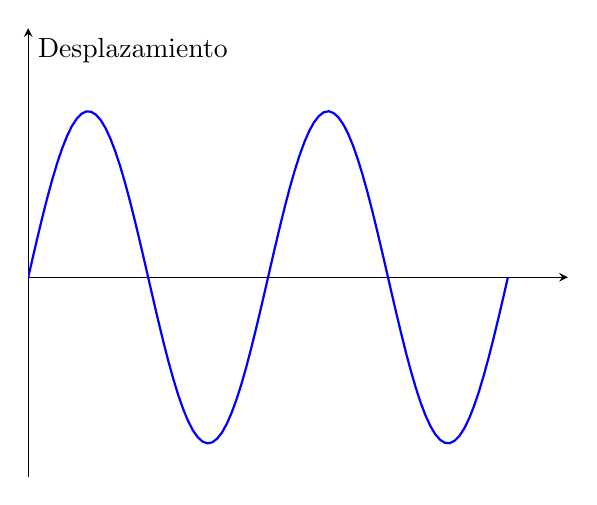
\begin{tikzpicture}
  \begin{axis}[
    xmin=0,xmax=4.5*pi,
    ymin=-1.2,ymax=1.5,
    axis lines=middle,
    xtick={0},
    ytick={0},
    ylabel=Desplazamiento
    ]

    % Funcion senoidal
    \addplot[color=blue,samples=100,domain=0:4*pi,thick]{sin(deg(x))};
  \end{axis}
\end{tikzpicture}
